\thispagestyle{plain}
\chapter{Kosmische Strahlung}
In diesem Kapitel wird die kosmische Strahlung beschrieben, welche die Erdatmosphäre erreicht. Die kosmische Strahlung kann in eine primäre und eine sekundäre Komponente zerlegt werden. Die primäre Komponente beschreibt alle Teilchen, welche die Erdatmosphäre erreichen, wohingegen die sekundäre Komponente alle Teilchen sind, welche von dem Primärteilchen während der Propagation zur Erdoberfläche produziert werden und auf der Erde detektiert werden können.
\section{Ursprung der kosmischen Strahlung}
Kosmische Strahlung kann mehrere Ursprünge haben. Hierbei können die hochenergetischen Teilchen, welche die Erde erreichen in eine galaktische und extragalaktische Komponente aufgeteilt werden.

Niederenergetische kosmische Strahlung ($E<$\SI{50}{PeV}) kann in Supernova Überresten produziert werden. Innerhalb der Supernova kommt es zu einer Schock-Beschleunigung, wenn die Schockfront auf das interstellare Medium trifft.  Innerhalb der Schockfront und dem interstellaren Medium sind turbulente Magnetfelder vorhanden, wodurch die Teilchen abgelenkt werden können. Die hochenergetischen Teilchen der Schockfront können durch die turbulenten Magnetfelder mehrmals die Ebene zwischen Schockfront und dem interstellaren Medium passieren. Durch diesen stochastischen Prozess entsteht ein Energiespektrum, welches einem Potenzgesetz folgt, welche auch in der Natur beobachtet werden. Dieser Prozess der Beschleunigung wird auch Fermibeschleunigung erster Ordnung gennant, da Teilchen, welche den Schock passieren jedes mal einen Energiezuwachse von 
\begin{align}
\Delta E \propto \left(\frac{v}{c_0}\right)^1
\end{align}
erfährt.


Galak und extragalak.

Für extrem hochenergetische Teilchen ($E>$\SI{50}{EeV}) kann eine Beschleunigung nicht mehr in der Galaxis stattfinden. Gute Kandidaten für die Produktion von hochenergetischer kosmischer Strahlung sind aktive galaktische Kerne, welche auch AGN genannt werden. Diese aktiven galaktischen Kerne haben ein massives schwarzes Loch in ihrem Zentrum und sind von einem Staubtorus umgeben. Durch die Akkretion von Masse durch das schwarze Loch entsteht ein Jet, welcher Senkrecht zu der Staubtorus Ebene ist. In diesem Jet sind diffuse Magnetfelder vorhanden, wodurch Teilchen durch die Fermi-Beschleunigung erster Ordnung zu höheren Energien beschleunigt werden können. Eine weitere Möglichkeit hochenergetische Kosmische Strahlung zu produzieren, kann über die Fermi-Beschleunigung zweiter Ordnung erfolgen, jedoch ist dieser Prozess sehr ineffizient und die Anwendungen auf tatsächliche Quellen schwierig.




\section{Primäre kosmische Strahlung S.5}
\begin{figure}[!h]
    \centering
    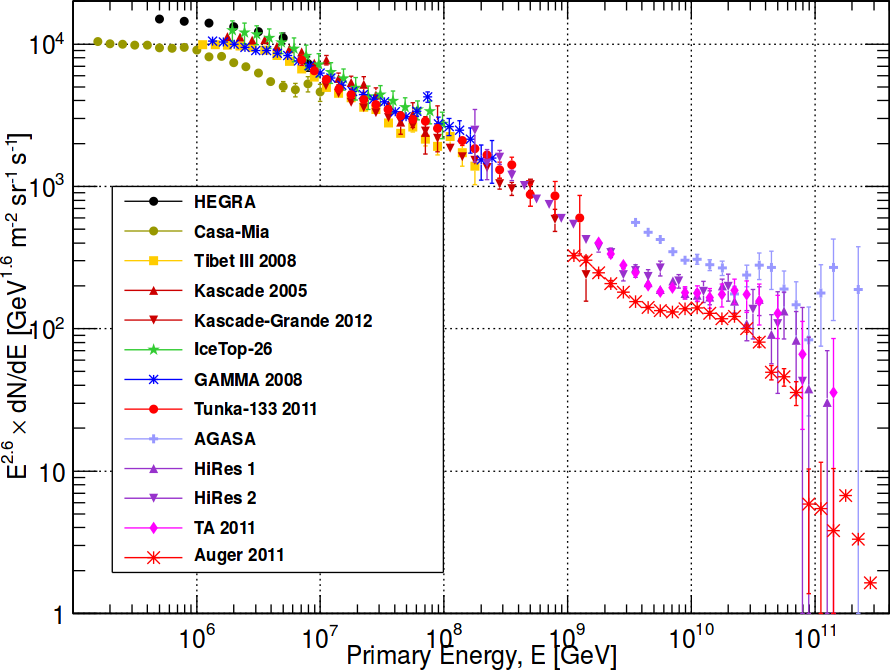
\includegraphics[width=0.7\textwidth]{./Plots/CR_Spectrum.png}
    \caption{Differentielles Spektrum der kosmischen Strahlung gemessen durch verschiedenen Exterimente.\ref{Paper} Dieses Spektrum ist mit der Energie, um einen Faktor von $E^{2.6}$ gewichtet. Dadurch sind das Knie ($\approx$\SI{3}{PeV}), das zweite Knie ($\approx$\SI{80}{PeV}) und die Ferse ($\approx$\SI{50}{EeV}) des Spektrums der Kosmischen Strahlung deutlich erkennbar.}
    \label{fig:SpecStrahl}
\end{figure}
\section{Sekundäre kosmische Strahlung S.2}
Bei der Propagation von hochenergetischen geladenen Teilchen oder Photonen in der Atmosphäre werden sekundäre Teilchen erzeugt. Diese sekundären Teilchen können hochenergetische Leptonen, Hadronen oder Leptonen sein, welche wiederum Teilchen erzeugen. Die sekundäre kosmische Strahlung kann in drei Komponenten unterteilt werden, welche als hadronische, myonische und elektromagnetische Komponenten bezeichnet werden.

Eine der am häufigsten produzierten Teilchen sind Pionen oder Kaonen, wobei im Folgenden nur auf Pionen eingegangen wird, da für Kaonen analoges gilt. Pionen können geladen als $\pi^{+/-}$ oder ungeladen als $\pi^0$ innerhalb der Atmospähre produziert werden. Aufgrund ihrer langen Lebensdauer von $\tau \approx 260$\,$\mu$s propagieren diese Teilchen durch die Atmosphäre und verlieren einen Teil ihrer Energie bevor sie Zerfallen. Die Dominanten Zerfallsprozesse für das negativ geladene und neutrale Pionen ergeben sich durch folgenden Zerfallsgleichungen:
\begin{align}
\pi^{-} &\rightarrow \mu^{-} + \nu_\mu \label{gl:PI} \\
\pi^0 &\rightarrow 2\gamma \label{gl:GAMMA}
\end{align}
Für das positiv geladene Pion in Gleichung \ref{gl:PI} entsteht ein positiv geladenes Myon und ein Anti-Myon Neutrino. Für höher energetische Proton-Proton-Kollisionen können kurzlebigere Teilchen Entstehen auf welche im Abschnitt \ref{ab:CRprompt} eingegangen wird. Der Zerfall der Pionen in Myonen stellt die Myonische Komponente dar, während der zerfall des ungeladenen Pions die elektromagnetische Komponente darstellt. Das Photon der elektromagnetischen Komponente produziert auf dem Weg zur erste Elektron-Positron-Paare, welche bis zur Erde progagieren.

In der hadronischen Komponente der kosmischen Strahlung werden Protonen, Neutronen, Pionen und andere Baryonen produziert. Diese können durch weitere Wechselwirkungen wieder Baryonen oder Pionen produzieren. Die Pionen können über Zerfallsprozesse in die anderen Komponenten der kosmischen Strahlung übergehen. 

Geladene Teilchen, welche sich mit einer Geschwindigkeit überhalb der Vakkuumlichtgeschwindigkeit bewegen, erzeugen niederenergetische Photonen auch \CH -Strahlung gennant. Diese Photonen können durch UV-Sensitive optische Elemente detektiert werden. Der Winkel der abgestrahlten Photonen bei der Erzeugung ist primär abhängig von dem Brechungsindes des Mediums in welchen sich das Teilchen bewegt. Für Luft beträgt der Winkel $\approx 3$°, wohingegen er bei Eis $\approx 40$° beträgt.
\section{Detektion}
Erreicht die kosmische Strahlung die Erde kann sie mit Hilfe von verschiedenen Prozessen detektiert werden. Im Nachfolgenden wird auf die verschiedenen Detektionsansätze für die verschiedenen Komponenten eingegangen.

Zur Detektion von hochenergetischen Photonen können Sateliten Experimente verwendet werden. Diese Experimente sind allerdings aufgrund ihrer geringen Detektionsfläche von einigen m$^2$ \ref{fermi} nicht im Stande den Fluss der höchst energetischten Photonen zu detektieren, da der Fluss dieser sehr gering ist. Eine andere Methode der Detektion von hochenergetischen Photonen sind Erdgebundene Teleskope. 
\section{Prompte Leptonen S.2}\label{ab:CRprompt}
Bei der Kollision von hochenergetischen Protonen mit Teilchen der Atmospähre können charmhaltige sekundärteilchen produziert werden. Diese Teilchen werden als prompte Komponente der kosmischen Strahlung bezeichnet, da diese sehr schnell zerfallen und somit keine Energie bei der propagation durch die Atmosphäre verlieren. Die Zerfallsdauer eines D-Mesonens ist mit $\tau \approx 1$\,ps sehr viel kleiner, als die des Pions. 